\def\lecturenumber{13}
\documentclass[11pt,a4paper]{article}
\usepackage[T1]{fontenc}
\usepackage[utf8]{inputenc}
\usepackage{lmodern}
\usepackage[margin=19mm,top=21mm,bottom=21mm,headheight=15pt]{geometry}
\usepackage{amsmath,amssymb,booktabs,array,graphicx,microtype}
\usepackage[dvipsnames]{xcolor}
\usepackage{enumitem,fancyhdr,listings,tcolorbox}
\usepackage[colorlinks=true,linkcolor=MidnightBlue,urlcolor=MidnightBlue]{hyperref}
\definecolor{courseblue}{HTML}{164B69}
\definecolor{pale}{HTML}{F0F5F7}
\pagestyle{fancy}
\fancyhf{}
\fancyhead[L]{\small\sffamily\color{courseblue}VALIDATED COMPUTING}
\fancyhead[R]{\small\sffamily Lecture \lecturenumber}
\fancyfoot[L]{\footnotesize Expanded lecture notes \textbullet\ October 2026}
\fancyfoot[R]{\footnotesize\thepage\ / 6}
\renewcommand{\headrulewidth}{0.4pt}
\setlength{\parindent}{0pt}
\setlength{\parskip}{5.5pt plus 1pt}
\setlength{\emergencystretch}{1.5em}
\setlist[itemize]{leftmargin=1.5em,itemsep=3pt,topsep=3pt}
\setlist[enumerate]{leftmargin=1.7em,itemsep=5pt,topsep=4pt}
\lstset{language=Python,basicstyle=\small\ttfamily,keywordstyle=\color{courseblue}\bfseries,
 commentstyle=\color{OliveGreen},stringstyle=\color{BrickRed},showstringspaces=false,
 columns=fullflexible,keepspaces=true,frame=single,rulecolor=\color{black!18},
 backgroundcolor=\color{black!2},aboveskip=6pt,belowskip=6pt,breaklines=true,
 xleftmargin=5pt,xrightmargin=5pt,framesep=5pt}
\newcommand{\R}{\mathbb R}
\newcommand{\fl}{\operatorname{fl}}
\newcommand{\abs}[1]{\left|#1\right|}
\newcommand{\heading}[2]{\section*{\color{courseblue}#1}\vspace{-4pt}{\small\sffamily\color{black!65}#2}\par\vspace{3pt}}
\newcommand{\opening}[2]{{\Large\sffamily\bfseries\color{courseblue}Lecture \lecturenumber\quad #1\par}\vspace{5pt}{\small #2}\par}
\newtcolorbox{question}[1]{colback=pale,colframe=courseblue!55,boxrule=0.4pt,
 arc=1mm,left=7pt,right=7pt,top=4pt,bottom=4pt,title={#1},fonttitle=\bfseries\small,
 coltitle=courseblue,colbacktitle=pale}
\newcommand{\reading}[1]{{\footnotesize\textbf{Reading and notebook.} #1\par}}
\hypersetup{pdfauthor={Validated Computing course},pdfsubject={Expanded introductory lecture notes with questions and exercises}}

\hypersetup{pdftitle={Lecture 13: Auditing a computational certificate}}
\begin{document}
\opening{Auditing a computational certificate}{Prerequisites: the validation methods used in the project; Lectures 09--12.\newline
Goal: connect a stated conclusion to its assumptions, decisive bounds, and complete decision record.}
\heading{1. Read the claim before reading the success message}{0--12 minutes: what evidence does this conclusion require?}
A computational certificate is a record supporting a precise mathematical
claim under stated assumptions. A status string, plot, or list of digits
is only part of that record. Review begins by restating the claim in terms
of a function, an input set, a domain or final time, and the quantifiers
being asserted: one point, every allowed input, one root, or all roots.

For example, ``there is exactly one root of $x^2-2$ in $[1,2]$, and it
lies in $[11/8,23/16]$'' is a reviewable claim. ``The root is correct''
does not specify which root, what error is bounded, or where uniqueness
holds. No amount of additional displayed precision repairs that omission.

\begin{center}
\begin{tabular}{p{0.23\linewidth}p{0.67\linewidth}}
\toprule
Part of the record & What a reviewer needs to identify\\
\midrule
Problem and inputs & Exact formula, domain, intended rationals or stored floats,
and any physical input uncertainty.\\[3pt]
Mathematical argument & The theorem or invariant and the hypotheses that make
it applicable to this problem.\\[3pt]
Arithmetic evidence & Exact or enclosing operations, working precision, and
the bounds used in the decisive comparisons.\\[3pt]
Scope and stopping & Local versus global claim, omitted or unresolved regions,
and the actual stopping criterion.\\[3pt]
Reproduction & Executable source, input data, environment, and saved results
that can be compared with a fresh run.\\
\bottomrule
\end{tabular}
\end{center}

Classify each premise by its source. Some are problem assumptions, such as
an ideal specular-reflection model. Others are analytic arguments, such as
continuous differentiability of a polynomial. Others are computed inequalities,
such as a derivative enclosure excluding zero. A reviewer should not expect
a numerical test to establish a modeling assumption or a file name to establish
a theorem hypothesis.

\begin{question}{Find the missing quantifier}
An author reports three narrow intervals containing roots. What further
evidence is needed for ``exactly three distinct roots on $[-3,4]$''?
Would reproducing the same intervals establish that no region was omitted?
\end{question}

Review the mathematical reasoning and code together. A reproducible error
remains an error. Conversely, failure of one proposed proof does not always
make the underlying claim false; it may mean that the available evidence
does not establish it. Distinguishing these findings makes the review useful
to an author who must repair either the computation or its interpretation.

Numerical certification still trusts the implementation, arithmetic libraries,
and their execution. These course certificates are not formal verification
of those implementations. Exact input descriptions and inspectable computations
make the trust assumptions easier to locate, not unnecessary.

\newpage
\heading{2. Recompute a small certificate from its recorded data}{12--30 minutes: a standalone rational checker}
For $f(x)=x^2-2$ on a positive interval $[a,b]$, the derivative enclosure
$[2a,2b]$ is exact. With midpoint $m$ and $c=f(m)$, interval Newton gives
$N=[m-\max(c/(2a),c/(2b)),m-\min(c/(2a),c/(2b))]$.
Lecture 09 proves that strict interior inclusion certifies exactly one root.
The following record stores rational endpoints as strings, preserving their
exact values independently of decimal display settings.
\begin{lstlisting}
from fractions import Fraction

record = {
    "problem": "x^2 - 2",
    "domain": ["1", "2"],
    "derivative": ["2", "4"],
    "newton": ["11/8", "23/16"],
    "claim": "exactly one root in domain",
}

def read_interval(values):
    return Fraction(values[0]), Fraction(values[1])

def verify_root_record(data):
    assert data["problem"] == "x^2 - 2"
    assert data["claim"] == "exactly one root in domain"
    a, b = read_interval(data["domain"])
    assert 0 < a < b
    slope_lower, slope_upper = read_interval(data["derivative"])
    assert (slope_lower, slope_upper) == (2*a, 2*b)
    center = (a + b) / 2
    value = center*center - 2
    quotients = [value/slope_lower, value/slope_upper]
    expected = (center-max(quotients), center-min(quotients))
    lower, upper = read_interval(data["newton"])
    assert (lower, upper) == expected
    assert a < lower <= upper < b
    return True

assert verify_root_record(record)
\end{lstlisting}

The checker is deliberately specific to one polynomial and one theorem.
It reconstructs the derivative and Newton calculations rather than trusting
the recorded claim. Polynomial smoothness is an analytic premise; the
checker does not infer it from the string naming the problem. The assertions
are classroom checks to run in ordinary Python with assertions enabled.

\begin{question}{Inspect the independent work done by the checker}
Which comparisons merely confirm the record's format or scope? Which
recompute mathematical evidence? Could a forged interior interval pass if
the line comparing it with \texttt{expected} were removed?
\end{question}

The exact rational result is $N=[11/8,23/16]\subset(1,2)$. The scalar
theorem supplies existence and uniqueness; the root-retention argument
locates that root inside $N$. A checker for arbitrary functions, machine
enclosures, or an entire global search would need substantially more evidence.

\newpage
\heading{3. Audit a summary that silently drops unresolved work}{30--46 minutes: a complete partition with an incomplete root search}
Consider $p(x)=(x+2)(x-1)(x-3)$ on $[-3,4]$. Here is a deliberately
partial, hand-constructed decision record. It is not the output of a full
search. Its left certificate can be justified by exact signs and a derivative
bound; its right side remains unresolved.
\begin{center}
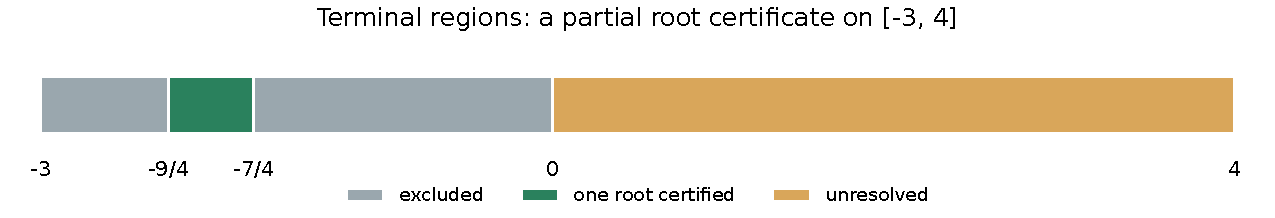
\includegraphics[width=0.94\linewidth]{figures/audit_partition.pdf}
\end{center}

On $[-3,-9/4]$, the three factors have fixed signs $-,-,-$, so $p<0$.
On $[-7/4,0]$ they have signs $+,-,-$, so $p>0$. These two regions contain
no root. On $X=[-9/4,-7/4]$, endpoint values are $-273/64$ and $209/64$.
Continuity proves existence. Evaluating $p'(x)=3x^2-4x-5$ with a sharp
square gives $[179/16,307/16]$, proving strict increase and uniqueness.
No decision has been supplied for $[0,4]$.
\begin{lstlisting}
certified = [(Fraction(-9, 4), Fraction(-7, 4))]
unresolved = [(Fraction(0), Fraction(4))]
excluded = [(Fraction(-3), Fraction(-9, 4)),
            (Fraction(-7, 4), Fraction(0))]
terminal = sorted(certified + unresolved + excluded)
assert terminal[0][0] == -3 and terminal[-1][1] == 4
for index in range(len(terminal) - 1):
    assert terminal[index][1] == terminal[index+1][0]
report = {
    "certified": certified,
    "unresolved": unresolved,
    "status": "incomplete",
    "all_roots_found": False,
}
\end{lstlisting}

An author who exports only the certified list and writes
\texttt{all\_roots\_found=True} has changed the conclusion. The defensible
report is: exactly one root lies in the certified interval; every other root
in the original domain lies in the unresolved region. The known roots $1$
and $3$ independently expose the omission, but the missing decision record
already prevents a completeness claim.

Coverage of terminal intervals is necessary for this partition argument.
It is not sufficient by itself: each exclusion and certification needs its
own justification. In a Newton search, contracted regions may instead be
removed by root retention; that record must explain why no root was lost.

\begin{question}{Repair the report at the correct layer}
Would more arithmetic bits correct the false completeness flag? What can
be honestly reported without further computation? What extra work would
support a count of all distinct roots in the original domain?
\end{question}

\newpage
\heading{4. Audit the trajectory's events and final time}{46--63 minutes: why a reflection list is not the whole certificate}
The mirror project uses ideal circles of radius $r=1/3$ at integer lattice
centres, initial position $(1/2,1/10)$, and initial velocity $(1,0)$.
The core target is time $T=3$. Specular reflection preserves the exact
speed, so the path travels total length $T$. Any collision centre must
therefore lie within $T+r$ of the initial point in each coordinate.

For these exact inputs the finite candidate list is
\[
                 -2\le i\le3,\qquad -3\le j\le3,
\]
with integer $i,j$: 42 centres. For example,
$\lceil1/2-3-1/3\rceil=-2$ and
$\lfloor1/2+3+1/3\rfloor=3$. Centres outside this rectangle cannot be
hit by time three. This analytic argument justifies finiteness; merely
drawing nearby mirrors would not establish it.

\textbf{Review each event decision.} Every candidate mirror needs either
a justified miss or an enclosing positive collision time. Suppose $T_i$
encloses one candidate flight time and $H$ encloses the remaining time.
The conservative selector accepts this collision only when
\[
 \sup T_i<\inf T_j\quad\hbox{for every other candidate hit }j,
 \qquad \sup T_i<\inf H.
\]
Overlapping intervals are inconclusive for these tests. A collision-free
finish requires all candidates to be justified misses or to satisfy
$\inf T_j>\sup H$. Unresolved geometry cannot be silently treated as a miss.

The previously hit mirror also needs a reason for being skipped. If the
exact collision point has outward normal vector $n$ of length $r$, and
the reflected direction $v$ satisfies $n\cdot v>0$, then for $t>0$
\[
            \|n+tv\|^2=r^2+2t(n\cdot v)+t^2\|v\|^2>r^2.
\]
Thus the ensuing straight segment departs from that circle. The invariant
that the actual collision point lies on the circle matters, even when its
rectangular coordinate enclosure includes off-circle points.

\textbf{Audit the clock as well as the position.} If the collision budget
is exhausted, the last certified state belongs to its recorded event-time
enclosure. It is not automatically a position enclosure at $T$. Propagating
it freely to the requested final time would assume that no unprocessed
collision occurs. The course's endpoint-reporting routine rejects an
incomplete trajectory rather than making that assumption.

\begin{question}{A horizon comparison to inspect}
The remaining time is enclosed by $[9/10,1]$ and a candidate flight time
by $[19/20,21/20]$. Which event happens first? What can the last certified
state still tell us if the time-order test is inconclusive?
\end{question}

Completion and accuracy are separate checks. After the final time is
certified, the project still requires coordinate and distance widths at
most $10^{-20}$. A completed trajectory with wider output has not yet met
that accuracy target; a narrow intermediate state has not yet reached $T$.

\newpage
\heading{5. Reproduce the evidence without changing its meaning}{63--76 minutes: serialization, fresh kernels, and a controlled defect}
Saved bounds must retain the mathematical input and output values used in
the proof. Exact rational strings are one simple serialization format.
Converting a narrow enclosure to a few rounded decimal digits may move an
endpoint inwards. Reopening the saved file should preserve the certificate,
not merely a display that looks similar to the original output.
\begin{lstlisting}
import json

payload = json.dumps(record, sort_keys=True)
restored = json.loads(payload)
assert verify_root_record(restored)

altered = dict(restored)
altered["newton"] = ["3/2", "8/5"]
try:
    verify_root_record(altered)
except AssertionError:
    print("Rejected: recorded interval disagrees with recomputation")
else:
    raise AssertionError("The altered record should have failed")
\end{lstlisting}

The altered interval is strictly inside $(1,2)$ but excludes $\sqrt2$.
A checker that tested only interior inclusion of the claimed interval
would accept a fabricated premise. Recomputing the Newton expression catches
the defect. A file hash would answer a different question: whether bytes
match a recorded version, not whether their mathematical contents are true.

A fresh-kernel run checks that the notebook does not depend on hidden
variables, stale imports, or cells executed in an unrecorded order. Record
the interpreter, arithmetic-library versions, precision settings, source
revision or source-file hashes, input encoding, and commands used. Keep
machine-specific paths out of the mathematical statement; identify the
actual files or records needed for reproduction.

For exact-rational computations, rerunning unchanged arithmetic should
reproduce the rational results. For verified numerical libraries, another
version may legitimately return different but valid outer endpoints.
Compare the exact input interpretation, decisive inequalities, and supported
claim as well as the printed digits. A discrepancy must be investigated
before treating two runs as interchangeable evidence.

\begin{question}{Design a reproduction check with a purpose}
Which failure would a fresh kernel reveal that a saved-output screenshot
might hide? Which failure would the rational checker reveal even if the
notebook reproduced its original output perfectly? Explain the limitation
of each check rather than treating either as universal validation.
\end{question}

Choose at least one successful example and one limiting example for review.
The latter checks whether the implementation preserves uncertainty and
reports its actual scope. A solver that always prints success can appear
convincing on easy cases while mishandling precisely the cases in which
validation is most needed.

Use the peer-audit notebook to record a cell or record reference, a concrete
finding, its effect on the claim, and a proposed correction. The author
should respond to each finding and update the final conclusion after rerunning
any affected computation. Preserve enough detail to see what was actually checked.

\newpage
\heading{6. Peer-review workshop and exercises}{76--90 minutes: audit in pairs; finish longer checks independently}
Spend two minutes restating a partner's claim, five minutes checking one
theorem premise and one scope decision, four minutes writing a finding and
an author response, and three minutes agreeing on a corrected conclusion.
The full fresh-kernel reproduction can be prepared before class or completed
afterward; do not describe an unperformed rerun as part of the review.

\begin{enumerate}
\item \textbf{A false implication.} An author encloses $x^2+1$ by $[0,2]$
on $[-1,1]$ and concludes that a root exists because zero is included.
Identify the incorrect inference. Give a better enclosure and state the
result it proves. Is the original wide enclosure itself invalid?

\item \textbf{Reconstruct a local certificate.} Verify the endpoint signs
and derivative bound for the negative cubic root on page 3. Check the
terminal partition, then write the strongest supported statement about
roots on $[-3,4]$ without resolving $[0,4]$.

\item \textbf{A correct answer with an incomplete proof.} Two disjoint
boxes each carry a valid local system certificate. The author concludes
that these are all real solutions. What additional argument is needed?
Explain why the supplied evidence need not show the conclusion is false.

\item \textbf{A partial trajectory.} A run stops after one certified
reflection with an inconclusive status. Its position widths are below
$10^{-20}$. Does it meet the project's final-time requirement? Name the
fields needed to distinguish the supported state from the requested endpoint.

\item \textbf{A certificate after export.} The rational interval
$[1/3-1/10000,1/3+1/10000]$ is exported by rounding both endpoints to
\texttt{0.333}. Does the reopened interval still enclose $1/3$? Give
an exact serialization and an outward-rounded three-decimal alternative.
\end{enumerate}

\textbf{Selected checks.} Exercise 1: zero inclusion does not prove a
root; the sharp-square form gives $[1,2]$, excluding zero. Exercise 2:
the signs are $-273/64$ and $209/64$, and the positive derivative bound
is $[179/16,307/16]$. Exactly one root is certified on the left, and all
other possible roots remain in $[0,4]$. Exercise 3 requires a global
exclusion or exhaustive search argument. Exercise 4 does not establish
arrival at time three; retain elapsed time, requested time, status, reason,
and the last certified state. Exercise 5: the singleton fails; exact
fraction endpoints or the outward interval $[0.333,0.334]$ are safe.

\begin{question}{Choose the review outcome and justify it}
Use \emph{supported under stated assumptions} when the checked argument
supports the scoped claim; \emph{needs correction} for a specific defect;
and \emph{inconclusive} when the available method or evidence does not settle
the request. State which checks you performed and what remains open.
\end{question}

An effective finding names the missing premise or wrong comparison and
explains its consequence. ``Use more precision'' is not a correction for
an omitted region, an unproved event order, or a changed input model.

\reading{Companions: \texttt{notebooks/13\_certificate\_audit.ipynb},
\texttt{assignments/peer\_audit.ipynb}, and the rubric in \texttt{projects/README.md}.
Review the theorem used in the submitted project. For mirrors, the course
adapts SIAM Challenge Chapter 2 to a shorter final-time target.}
\end{document}
